\chapter{Data Sources}\label{Chp:ref:data sources}

At the source of every inversion is data in the form of gravity anomaly or
magnetic flux density values for at least a part of the region of interest.
These usually come from surveys and are preprocessed to correct for various
factors and distortions.
This chapter provides an overview of the classes related to data input for
inversions.

\section{Overview}
The inversion module comes with a number of classes that can read gridded
(raster) data on a 2-dimensional plane from file or provide artificial values
for testing purposes. These classes all derive from the abstract
\class{DataSource} class and override methods that return information about
the data and the values themselves.
The \class{DomainBuilder} class is responsible for creating an \escript domain
with a suitable grid spacing and spatial extents that include all data sources
attached to it (see Figure~\ref{fig:domainBuilder}).
%
\begin{figure}[ht]
    \centering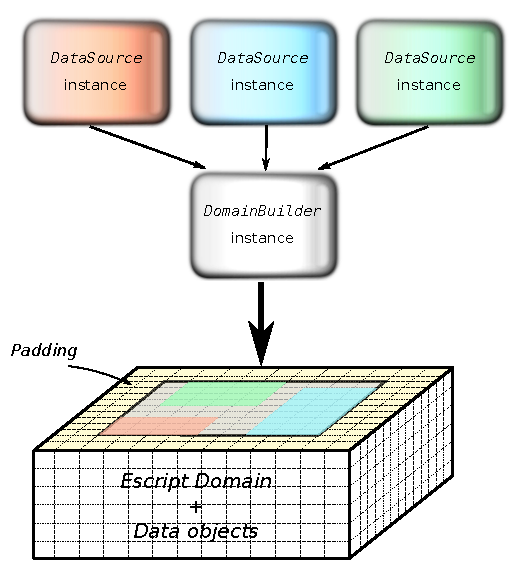
\includegraphics{domainbuilder}
    \caption{\class{DataSource} instances are added to a \class{DomainBuilder}
        which creates a suitable domain and \Data objects for the inversion}
    \label{fig:domainBuilder}
\end{figure}
%
Notice that in the figure there are cells in the region of interest that are
not covered by any data source instance.
Ideally, all data sources used for an inversion have the same spatial resolution
and are spatially adjacent so that all cells have a value but this is not a
requirement.


\section{Domain Builder}\label{Chp:ref:domain builder}
Every inversion requires one \class{DomainBuilder} instance which creates and
holds a reference to the \escript domain as well as associated \Data objects for
the input data used for the inversion.
The class has the following public methods:

\begin{classdesc}{DomainBuilder}{\optional{dim=3, }\optional{reference_system=\None}}
Constructor for the domain builder. \member{dim} sets the dimensionality of the
target domain and must be 2 or 3. By default a 3-dimensional domain is created.
\member{reference_system} defines the reference coordinate system to be used, see Section~\ref{sec:ref:reference systems}.
If not present the Cartesian reference coordinate system is used.
\end{classdesc}

\begin{methoddesc}[DomainBuilder]{addSource}{source}
adds survey data \member{source} (a \class{DataSource} object) to the domain
builder. The dimensionality of the data must be less than or equal to the
domain dimensionality. The reference coordinate system of the \class{DataSource}
must match the reference coordinate system of this class. 
The \member{source} must be defined for the same reference coordinate system to be used, see Section~\ref{sec:ref:reference systems}.
\end{methoddesc}

\begin{methoddesc}[DomainBuilder]{setVerticalExtents}{%
\optional{depth=40000.}%
\optional{, air_layer=10000.}%
\optional{, num_cells=25}}
sets the parameters for the vertical dimension of the domain. The parameter
\member{depth} specifies the thickness in meters of the subsurface layer
($-x_2^{min}$ in Figure~\ref{fig:cartesianDomain}).
The default value of $40$ km is usually appropriate. Similarly, the
\member{air_layer} parameter defines the buffer zone thickness above the surface
($x_2^{max}$ in Figure~\ref{fig:cartesianDomain}) which should be a few
kilometres to avoid artefacts in the inversion.
The number of elements (or cells) in the vertical dimension is set with the
\member{num_cells} parameter. Consider the size and resolution of your datasets,
the total vertical length (=\member{depth}+\member{air_layer}) and available
compute resources when setting this value.
\end{methoddesc}

\begin{methoddesc}[DomainBuilder]{setFractionalPadding}{%
\optional{pad_x=\None}%
\optional{, pad_y=\None}}
sets the amount of padding around the dataset as a fraction of the dataset side
lengths if the reference coordinate system is Cartesian. 
For example, calling \member{setFractionalPadding(0.2, 0.1)} with a data source
of size $10000 \times 20000$ meters will result in the padded data set size $14000 \times 24000$ meters
(that is $10000 \times (1+2 \times 0.2)$ and $20000 \times (1+2 \times 0.1)$).
By default no padding is applied and \member{pad_y} is ignored for 2-dimensional
domains.
\end{methoddesc}

\begin{methoddesc}[DomainBuilder]{setFractionalPadding}{%
\optional{pad_lat=\None}%
\optional{, pad_lon=\None}}
sets the amount of padding around the dataset as a fraction of the dataset side
lengths if the reference coordinate system is not Cartesian.
For example, calling \member{setFractionalPadding(0.2, 0.1)} with a data source
of size $10 \times 20$ degree will result in the padded data set size $14 \times 24$ degree
(that is $10 \times (1+2 \times 0.2)$ and $20 \times (1+2 \times 0.1)$).
By default no padding is applied and \member{pad_lon} is ignored for 2-dimensional
domains.
\end{methoddesc}

\begin{methoddesc}[DomainBuilder]{setPadding}{%
\optional{pad_x=\None}%
\optional{, pad_y=\None}}
sets the amount of padding around the dataset in absolute length units.
The final domain size will be the length in x (in y) of the dataset plus twice
the value of \member{pad_x} (\member{pad_y}). The arguments must be non-negative.
By default no padding is applied and \member{pad_y} is ignored for 2-dimensional
domains. This function can be used for Cartesian reference coordinate system  only.
\end{methoddesc}

\begin{methoddesc}[DomainBuilder]{setElementPadding}{%
\optional{pad_x=\None}%
\optional{, pad_y=\None}}
sets the amount of padding around the dataset in number of elements (cells),
if the reference coordinate system is Cartesian. 
When the domain is constructed \member{pad_x} (\member{pad_y}) elements are
added on each side of the x- (y-) dimension in case of a Cartesian reference system. The arguments must be non-negative integers.
By default no padding is applied and \member{pad_y} is ignored for 2-dimensional
domains.
\end{methoddesc}

\begin{methoddesc}[DomainBuilder]{setElementPadding}{%
\optional{pad_lat=\None}%
\optional{, pad_lon=\None}}
sets the amount of padding around the dataset in number of elements (cells) if the the reference coordinate system is not Cartesian.
When the domain is constructed \member{pad_lat} (\member{pad_lon}) elements are
added on each side of the latitudinal (longitudinal) dimension. The arguments must be non-negative integers.
By default no padding is applied and \member{pad_lon} is ignored for 2-dimensional
domains.
\end{methoddesc}

\begin{methoddesc}[DomainBuilder]{fixDensityBelow}{%
\optional{depth=\None}}
defines the depth below which the density anomaly is fixed to zero.
This method is only useful for inversions that involve gravity data.
\end{methoddesc}

\begin{methoddesc}[DomainBuilder]{fixSusceptibilityBelow}{%
\optional{depth=\None}}
defines the depth below which the susceptibility anomaly is fixed to zero.
This method is only useful for inversions that involve magnetic data.
\end{methoddesc}

\begin{methoddesc}[DomainBuilder]{getGravitySurveys}{}
returns a list of all gravity surveys added to the domain builder. See
\member{getSurveys()} for more details.
\end{methoddesc}

\begin{methoddesc}[DomainBuilder]{getMagneticSurveys}{}
returns a list of all magnetic surveys added to the domain builder. See
\member{getSurveys()} for more details.
\end{methoddesc}

\begin{methoddesc}[DomainBuilder]{getSurveys}{datatype}
returns a list of surveys of type \member{datatype} available to this domain
builder. In the current implementation each survey is a tuple of two \Data
objects, the first containing anomaly values and the second standard error
values for the survey.
\end{methoddesc}

\begin{methoddesc}[DomainBuilder]{getDomain}{}
returns an \escript domain (see~\cite{ESCRIPT}) suitable for running inversions
on the attached data sources.
The first time this method is called the target parameters (such as resolution,
extents and number of elements) are computed, and the domain is created.
Subsequent calls return the same domain instance so calls to
\member{setPadding()}, \member{addSource()} and other methods that influence
the domain will fail once \member{getDomain()} is called the first time.
\end{methoddesc}

\begin{methoddesc}[DomainBuilder]{getReferenceSystem}{}
returns the reference coordinate system
\end{methoddesc}

\begin{methoddesc}[DomainBuilder]{setBackgroundMagneticFluxDensity}{B}
sets the background magnetic flux density $B=(B_{North},B_{East},B_{Vertical})$
which is required for magnetic inversions.
$B_{East}$ is ignored for 2-dimensional magnetic inversions.
\end{methoddesc}

\begin{methoddesc}[DomainBuilder]{getBackgroundMagneticFluxDensity}{}
returns the background magnetic flux density $B$ set via
\member{setBackgroundMagneticFluxDensity()} in a form suitable for the inversion.
There should be no need to call this method directly.
\end{methoddesc}

\begin{methoddesc}[DomainBuilder]{getSetDensityMask}{}
returns the density mask \Data object which is non-zero for cells that have a
fixed density value, zero otherwise.
There should be no need to call this method directly.
\end{methoddesc}

\begin{methoddesc}[DomainBuilder]{getSetSusceptibilityMask}{}
returns the susceptibility mask \Data object which is non-zero for cells that
have a fixed susceptibility value, zero otherwise.
There should be no need to call this method directly.
\end{methoddesc}

\section{\class{DataSource} Class}\label{sec:ref:DataSource}

Data sources added to a \class{DomainBuilder} must provide an implementation for
a few methods as described in the class template \class{DataSource} from
the \module{esys.downunder.datasources} module:

\begin{classdesc}{DataSource}{\optional{reference_system=\None}}
Base constructor which initializes members and should therefore be invoked by
subclasses. Subclasses may then use the member \member{logger} to print any
output. \member{reference_system} defines the reference coordinate system to be used, see Section~\ref{sec:ref:reference systems}.
If not present the Cartesian reference coordinate system is used.
\end{classdesc}

\begin{methoddesc}[DataSource]{getDataExtents}{}
This method should be implemented to return a tuple of tuples
( (x0, y0), (nx, ny), (dx, dy) ), where (x0, y0) denote the UTM coordinates of
the data origin, (nx, ny) the number of data points, and (dx, dy) the spacing
of data points in a Cartesian reference system is used. Otherwise 
the data origin and the spacing refer to latitudinal and longitudinal coordinates.
\end{methoddesc}

\begin{methoddesc}[DataSource]{getDataType}{}
Subclasses must return \class{DataSource}.\member{GRAVITY} or
\class{DataSource}.\member{MAGNETIC} depending on the type of data they provide.
\end{methoddesc}

\begin{methoddesc}[DataSource]{getSurveyData}{domain, origin, NE, spacing}
This method is called by the \class{DomainBuilder} to retrieve the actual survey
data in the form of \Data objects on the \member{domain}.
Data sources are responsible to map or interpolate their data onto the domain
which has been constructed to fit the data.
The domain \member{origin}, number of elements \member{NE} and element
\member{spacing} are provided as tuples or lists to aid with interpolation.
\end{methoddesc}

\begin{methoddesc}[DataSource]{getUtmZone}{}
Must be implemented to return the UTM zone that corresponds to the location of
this data set as returned by \member{getDataExtents}.
\end{methoddesc}

\begin{methoddesc}[DataSource]{setSubsamplingFactor}{factor}
Notifies the data source that data should be subsampled by \member{factor}.
This method does not need to be overwritten.
See \member{getSubsamplingFactor()} for an explanation.
\end{methoddesc}

\begin{methoddesc}[DataSource]{getSubsamplingFactor}{}
Returns the subsampling factor which was set by \member{setSubsamplingFactor()}
or $1$ which indicates that no subsampling is requested.
Data sources that support subsampling (or interleaving) of their data should use
this method to query the subsampling factor before returning surveys via
\member{getSurveyData}. If supported, the factor should be applied in all
dimensions. For example, a 2-dimensional dataset with 300 x 150 data points
should be reduced to 150 x 75 data points when the subsampling factor equals $2$.
Subsampling becomes important when the survey data resolution is too fine or
when using data with varying resolution in one inversion.
Note that data sources may choose to ignore the subsampling factor if they
don't support it.
\end{methoddesc}

\begin{methoddesc}[DataSource]{getReferenceSystem}{}
returns the reference coordinate system
\end{methoddesc}

\vspace{1em}\noindent The \module{esys.downunder.datasources} module contains the following helper
functions:

\begin{funcdesc}{LatLonToUTM}{longitude, latitude%
\optional{, wkt_string=\None}}
converts one or more (longitude,latitude) pairs to the corresponding (x,y)
coordinates in the \emph{Universal Transverse Mercator} (UTM) projection.
This function requires the \module{pyproj} module for conversion and the
\module{gdal} module to parse the \member{wkt_string} parameter if supplied.
The \member{wkt_string} parameter may describe the coordinate system used
for the input values as a \emph{Well-known Text} (WKT) string.
\end{funcdesc}

\subsection{ER Mapper Raster Data}\label{sec:ref:DataSource:ERM}
\emph{ER Mapper} files that contain 2-dimensional raster data may be used for
inversions through the \class{ErMapperData} class which is derived from
\class{DataSource}. Date are given in latitudinal and longitudinal coordinates and if
a Cartesian reference coordinate system is used are mapped using the appropriate  (UTM) projection. 
Generally, these datasets contain two files~\cite{ERMAPPER}, a header file and a data file.
The former usually has the \texttt{.ers} file extension and is a text file that
describes the data format, size, coordinate system used etc.
The data file usually has the same file name but no extension.
Note, that the current implementation may not work with all \emph{ER Mapper}
datasets. For example, the only cell type understood is \emph{IEEE4ByteReal}
at the moment.
To run inversions on a \emph{ER Mapper} dataset use the following constructor:
\begin{classdesc}{ErMapperData}{data_type, headerfile%
\optional{, datafile=\None}%
\optional{, altitude=0.}%
\optional{, error=\None}%
\optional{, scale_factor=\None}%
\optional{, null_value=\None}
\optional{, reference_system=\None}}
Creates a new data source from \emph{ER Mapper} data.
The parameter \member{data_type} must be one of
\class{DataSource}.\member{GRAVITY} or \class{DataSource}.\member{MAGNETIC}
depending on the type of data, \member{headerfile} is the name of the header
file while \member{datafile} specifies the name of the data file.
The parameter \member{datafile} can be left blank if the name is identical to
the header file except for the file extension.
The \member{altitude} parameter can be used to shift a 2-dimensional slice of
data vertically within a 3-dimensional domain.
Use \member{error} to set the (constant) measurement error with the same units
used by the measurements. By default a value of $2$ units is assumed which
equals $0.2 \; mgal$ or $2 \; nT$ depending on the data type.
Since ER Mapper files do not store any information about data units or scale
the \member{scale_factor} may be used to provide this information.
If not set, gravity data is assumed to be given in $\frac{\mu m}{sec^2}$ while
magnetic data is assumed to be given in $nT$.
Finally, the \member{null_value} parameter can be used to override the value
for the areas to be ignored (see Section~\ref{SEC:P1:GRAV:REMARK:DATAHOLES})
which is usually provided in the ER Mapper header file.
\member{reference_system} defines the reference coordinate system to be used, see Section~\ref{sec:ref:reference systems}.
If not present the Cartesian reference coordinate system is used. In the current implementation any
coordinate system specified in the file is ignored.
\end{classdesc}

\subsection{NetCDF Data}\label{sec:ref:DataSource:NETCDF}
The \class{NetCdfData} class from the \module{esys.downunder.datasources} module
provides the means to use data from \netcdf files~\cite{NETCDF} for inversion.
Currently, files that follow the \emph{Climate and Forecast (CF)}\footnote{%
\url{http://cf-pcmdi.llnl.gov/documents/cf-conventions/latest-cf-conventions-document-1}}
and/or the \emph{Cooperative Ocean/Atmosphere Research Data Service (COARDS)}\footnote{%
\url{http://ferret.wrc.noaa.gov/noaa_coop/coop_cdf_profile.html}} metadata
conventions are supported.
The example script \examplefile{create_netcdf.py} demonstrates how a compatible
file can be generated from within \Python (provided the \module{scipy} module
is available).
To plot such an input file including coordinates and legend using
\emph{matplotlib}~\cite{matplotlib} see the script \examplefile{show_netcdf.py}.
The interface to \class{NetCdfData} looks as follows:

\begin{classdesc}{NetCdfData}{datatype, filename%
\optional{, altitude=0.}%
\optional{, data_variable=\None}%
\optional{, error=\None}%
\optional{, scale_factor=\None}%
\optional{, null_value=\None}
\optional{, reference_system=\None}}
Creates a new data source from compatible \netcdf data.
The two required parameters are \member{datatype}, which must be one of
\class{DataSource}.\member{GRAVITY} or \class{DataSource}.\member{MAGNETIC}
depending on the type of data, and \member{filename} which is the name of the
file containing the data.
The \member{altitude} parameter can be used to shift a 2-dimensional slice of
data vertically within a 3-dimensional domain.
Set the \member{data_variable} parameter to the name of the \netcdf variable
that contains the measurements unless there is only one data variable in the
file in which case the parameter can be left empty.
Use \member{error} to set the (constant) measurement error with the same units
used by the measurements or the name of the \netcdf variable that contains this
information. By default a value of $2$ units is assumed which equals
$0.2 \; mgal$ or $2 \; nT$ depending on the data type.
The current implementation does not use the units attribute (if available)
within the \netcdf file. Use the \member{scale_factor} argument to provide this
information instead.
If not set, gravity data is assumed to be given in $\frac{\mu m}{sec^2}$ while
magnetic data is assumed to be given in $nT$.
Finally, the \member{null_value} parameter can be used to override the value
for the areas to be ignored (see Section~\ref{SEC:P1:GRAV:REMARK:DATAHOLES})
which is usually provided in the \netcdf file. \member{reference_system} defines the reference coordinate system to be used, see Section~\ref{sec:ref:reference systems}.
If not present the Cartesian reference coordinate system is used. In the current implementation any
coordinate system specified in the file is ignored.
\end{classdesc}

\subsection{Synthetic Data}
As a special case the \module{esys.downunder.datasources} module contains
classes to generate input data for inversions by solving a forward model with
user-defined reference data.
The main purpose of using synthetic data is to test the capabilities of the
inversion module or for tracking down problems.

The base class for synthetic data which is derived from \class{DataSource}
has the following interface:

\begin{classdesc}{SyntheticDataBase}{datatype%
\optional{, DIM=2}
\optional{, number_of_elements=10}
\optional{, length=1*U.km}def SphericalReferenceSystem(R=6378137.0*U.m):
\optional{, B_b=\None}
\optional{, data_offset=0}
\optional{, full_knowledge=\False}}
Base class to define reference data based on a given property distribution
(density or susceptibility). Data are collected from a square region of
vertical extent \member{length} on a grid with \member{number_of_elements}
cells in each direction.
The synthetic data are constructed by solving the appropriate forward problem.
Data can be sampled with an offset from the surface at $z=0$ or using the
entire subsurface region.
\end{classdesc}

\vspace{1em}\noindent The only additional method which needs to be implemented
in subclasses is
\begin{methoddesc}[SyntheticDataBase]{getReferenceProperty}{
\optional{domain=\None}}
Returns the reference \Data object that was used to generate the gravity or
susceptibility anomaly data. The \member{domain} argument must be present
when this method is called for the first time but not necessarily in
subsequent calls.
\end{methoddesc}

\vspace{1em}\noindent Two synthetic data providers are currently available.
The class \class{SyntheticData} defines synthetic gravity or magnetic anomaly
data based on a harmonic
\begin{equation}\label{eq:synthdata}
    k=A\cdot sin\left(\pi \frac{n_D}{D} (z+\Delta z)\right) \cdot%
        sin\left(\pi \frac{n_L}{L} (x - x_0)\right)
\end{equation}
where $A$ is the amplitude, $n_D$, $n_L$ denote the number of oscillations in
the vertical and lateral direction, respectively, while $D$ and $L$ is the
depth and side length for the data, respectively.
The second data provider class is \class{SyntheticFeatureData} which takes a
list of \class{SourceFeature} objects that define the anomaly and is thus more
generic.
The constructors are defined as follows:

\begin{classdesc}{SyntheticData}{datatype%
\optional{, n_length=1}
\optional{, n_depth=1}
\optional{, depth_offset=0.}
\optional{, depth=\None}
\optional{, amplitude=\None}
\optional{, DIM=2}
\optional{, number_of_elements=10}
\optional{, length=1*U.km}
\optional{, B_b=\None}
\optional{, data_offset=0}
\optional{, full_knowledge=\False}
\optional{, spherical=\False}}
The arguments \member{n_length}, \member{n_depth}, \member{depth_offset},
\member{depth}, and \member{amplitude} correspond to the respective symbols in
Equation~\ref{eq:synthdata}. The remaining arguments are passed to the parent
class (\class{SyntheticDataBase}) and described there.
If \member{depth} is not set the depth of the domain is used.
The argument \member{amplitude} may be left unset as well in which case a
default value is used ($200 \frac{kg}{m^3}$ for gravity and $0.1$ for magnetic
data).
\end{classdesc}

\begin{classdesc}{SyntheticFeatureData}{datatype, features%
\optional{, DIM=2}
\optional{, number_of_elements=10}
\optional{, length=1*U.km}
\optional{, B_b=\None}
\optional{, data_offset=0}
\optional{, full_knowledge=\False}
\optional{, spherical=\False}}
The only new argument is \member{features} which is a list of
\class{SourceFeature} objects to be included in the data preparation.
All other arguments are passed on to the parent class (see there).
\end{classdesc}

\begin{classdesc}{SourceFeature}{}
A feature adds a density/susceptibility distribution to (parts of) a domain of
a synthetic data source, for example a layer of a specific rock type or a
simulated ore body. This base class is empty and only provides the skeleton
for subclasses which need to implement the following two methods:
\end{classdesc}

\begin{methoddesc}[SourceFeature]{getValue}{}
Returns the value for the area covered by mask. It can be constant or a \Data
object with spatial dependency.
\end{methoddesc}

\begin{methoddesc}[SourceFeature]{getMask}{x}
Returns the mask of the region of interest for this feature. That is, mask is
non-zero where the value returned by \member{getValue()} should be applied,
zero elsewhere.
\end{methoddesc}

